\documentclass[11pt]{article}

\usepackage[margin=25mm]{geometry}
\usepackage{times}

\usepackage[
backend=bibtex,
style=numeric
]{biblatex}
\usepackage{graphicx}

\addbibresource{proposal.bib}

\author{Stephen Livermore-Tozer}
\title{Research Proposal: Practical Algorithmic Co-composition}

\begin{document}
	\maketitle
	
	\section{Case for Support}
	
	\subsection{Overview}
	
%	Although a reasonable volume of research has been committed to producing ``creative'' artificial intelligence for the creation of art, there is currently very little to show for it in terms of practical applications. One of the key reasons for this is that, as in many extremely hard problems that depend on experience and intuition, machines are still far from outperforming skilled humans in the general case. This is to be expected as the technology is still emerging and somewhat immature, but the currently available technology may still be suitable to start producing real world results when focused on the right task.
	
	The research being put forward by this proposal is directed towards the development of an algorithm capable of performing a large subset of the skills used in song composition. This particular work can be differentiated from other algorithmic composition research in that instead of writing original compositions independently, it will perform interactive composition with a human compose, acting as a co-composer. By doing so it is possible for a host application perform a significant share of the work during composition without being required to single-handedly tackle the full creative scope of the task; this approach addresses many of the shortcomings of current composition algorithms in the context of a practical implementation. 
	
	The expected gains for a successful application of the proposed technology are potentially great, as it stands to both profit from and bolster the music industry through the introduction of a unique and powerful tool for composition. This research is particularly relevant at this point in time, as the music industry is currently undergoing drastic changes as a result of technology and holds an uncertain future; a successful application of this research could have a powerful impact for artists and record labels alike.
	
	The main novelty of this research as compared to other algorithmic composition research is the goal towards which it is directed, and the heavy emphasis on enabling a practical application in its methodology. This research will therefore build heavily upon the existing literature, focusing on adapting it to achieve new results with the addition of user interaction and a more concrete set of objectives. 
	
	The key challenges that will be tackled by this research project can thus be summarised as:
	\begin{itemize}
		\item Mapping out the range of potential users for an algorithmic co-composition application and their desired uses for such an application.
		\item Identifying the means by which automation can be used to augment composition, comprehensively covering the set of tasks that may be achieved feasibly by known algorithmic composition methods, and assessing their potential value in real-world use cases.
		\item Creating design documents that specify a model for algorithmic co-composition that maximizes positive impact to the user based on data obtained through research.
		\item Implementing a working prototype co-composition application built according to the designs given as part of this research
	\end{itemize}
	
	Success in these areas would cleanly pave the way to practical algorithmic co-composition. This would be a groundbreaking step forward within the greater field of algorithmic composition, as to date such algorithms have served purely experimental or demonstrative purposes; involving an application directly in the real-world creative process of composition would provide enormous benefits to the field, in terms of useful research data, economic incentive, and public interest. 
	
	\subsection{Background}
	
	The use of technology in music composition has grown greatly in recent years. With the advent of software synthesizers, DAWs, and the MIDI format, the PC has become a powerful professional tool for composing and editing music. The impact that this has had on the music industry has been extraordinary, with much more power being put in the hands of independent and amateur producers; combined with the platform for promotion and distribution provided by the internet this has resulted in a greatly increased number of independent artists establishing a public presence and earning a profit from their work.
		
	Algorithmic composition as a field has captured the interest of many researchers, but currently remains highly impractical. There are many limitations to the currently used algorithms, and while partial successes have been made there is no current real-world use case for these systems. The goal of the majority of the existing body of work is to design a complete algorithmic composer of equal or comparable ability to a human composer. Although a great deal of progress has been made towards this goal however, it may not be the most direct route to an algorithmic composer that serves a practical purpose. 
	
	The most cutting-edge algorithmic composition systems currently are used to produce music for popular consumption. One of the most successful and well-known of these is Iamus, a supercomputer running software based on the Melomics system \cite{diaz2011composing}. Iamus uses evolutionary algorithms to write music according to a set of rules provided by its operators, which are intended to create contemporary classical music. The Melomics system has been further used to create large collections of music with a variety of styles, a repository of which is published and free to access online. Each of these collections are specialized for a particular purpose, such as aiding sleep or reducing anxiety. This system currently stands at the forefront of industrial-level algorithmic composition, being the only current example that directly creates content for the public with the potential for commercialization. It is still quite specialized in its use however - the majority of the music is not written for artistic appreciation, and the remainder of its music has had mixed responses from critics and little to no popular success. This is only to be expected given the complexity of producing popular music for a contemporary audience, but it illustrates well the infeasibly high difficulty of completing this task with current technological means. 
	
	% Continuation
	Algorithmically expanding an existing piece of music is also a fairly commonly attempted task. The particular type of expansion varies between works; some of the most common are harmonization, counterpoint, and directly combining with other melodies. These tasks are all important aspects of composition, yet are constrained enough for AI to perform reasonably well. Although there has been no real adoption of these algorithms by actual composers, some of the more successful cases have been assessed by experts as being competent at a basic level.
	% TODO: This seriously needs a citation, you'll probably need to comb the survey for 2 or 3 examples
	These 
	
%	\subsection{Not final}
%	
%	% Rule based systems
%	The earliest attempts at algorithmic composition were not knowledge-based, but rule-based. Musical experts would encode sets of compositional rules and constraints into code, which would then generate scores that followed these rules. Implementations of this method have been able to produce some interesting and occasionally powerful results. However, they are noted to be very ``brittle'', meaning that they tend to perform very poorly outside of certain cases. Performance improves slightly in specific subtasks, such as harmonization, but so far no suitable results have been produced.
%	
%	% Machine learning
%	Machine learning was introduced to composition during its earliest days, with the use of simple models such as Markov chains trained on small numbers of songs to generate rhythm \cite[]{pinkerton1956information}. These attempts tended to produce very low quality or simple output. The reasons for this include lack of processing power, lack of data sources, and the use of fairly unsophisticated methods. 
%	
%	More advanced approaches began to emerge decades based on the use of neural networks trained on a set of melodies to generate new melodies \cite[]{todd1989connectionist}. These methods still performed quite poorly in practise, but demonstrated more versatility and produced better subjective results than earlier attempts. Since then many more modern adaptations have been made to previous methods, such as using evolutionary search or learning rules from data. However, the results given by AI in pure composition are still quite poor according to subjective evaluation. 
%	
%	% Varied attempts
%	With this inadequacy of AI in its current state, most research is focused on specific subtasks of composition. These include tasks such as harmonization for specific genres or styles \cite{mcintyre1994bach}, measuring distance or `similarity' between musical objects \cite{horner1991genetic}, and generation of chord progressions \cite{chemillier2004toward}. The current AI landscape is not sufficient to create a whole original composition, as there are many gaps and imperfections in the work accomplished so far. 
%	
	\subsection{Objectives}
	
	The broad goal of this research is to establish a real-world presence for algorithmic co-composition systems, by building industrial interest and taking the first direct step towards such a system. To achieve this, we will build towards the following objectives:
	%The goal of this research is to both determine a means to achieve a practical algorithmic co-composition system, and develop a first prototype for such a system. The objectives that should be satisfied for this research to be considered successful are as follows:
	\begin{enumerate}
		\item To map out the range of potential users for algorithmic co-composition systems and determine their respective needs for such a system. This information will be gathered from these potential users, and will be comprehensive enough for a full system design to be based on.
		\item To create a requirement specification for a framework for some particular kind of algorithmic co-composition. This specification will not necessarily be fully detailed to create a finished system with, but will define the necessary behaviours and acceptable limits of such a system. The type of co-composition defined by this specification will be selected so as to maximize overall user value while working within known feasibility (as determined by existing research).
		\item To design and implement a simple prototype algorithmic co-composition application. This application will be based on (but not necessarily exactly fitting to) the specification prepared as part of this work. This is expected to serve as a proof of concept for future developers, and will be used for testing 
		
	\end{enumerate}
		
	\subsection{Success Criteria}
	
	As the central goal of this research is to bring algorithmic co-composition (and by extension algorithmic composition) into practical usage, the success of this work should be judged by how well it is able to build the foundations for future work and establish a presence among developers and potential users. As such the criteria that should be met by this work are:
	\begin{enumerate}
		\item The 
	\end{enumerate}
	
	\subsection{Workpackages}
	
	The workpackages which comprise this research can be compared loosely to a single iteration of a software development project, with requirement gathering and specification, prototyping, and collecting user feedback. This is intentional, as this work should provide a solid foundation for algorithmic co-composition systems that developers or other researchers may build on. There are certain key differences however: rather than iteratively designing, building, and refining a product, we will be creating a framework. This is reflected in the ``loose'' nature of the deliverables, where many implementational details that would be essential in a full development cycle (such as testing, maintenance, or fully meeting the specification) are ignored; instead the deliverables are each valuable resources for anybody building an algorithmic co-composition system.
	
	\subsubsection*{WP1: User input and feedback}
	
	\noindent \textbf{Staff}:
	\smallskip
	
	PhD1, Smith Johnston
	
	\noindent \textbf{Research objective}:
	\smallskip
	
	The purpose of this primarily social science-based package is to gather and consolidate a comprehensive list of desired functionalities for the ideal use-cases of potential users. These requirements will be elicitated using information gathering methods broadly targeting the set of potential users, which include professional musicians/songwriters from across all domains of the music industry. Of these people, we will primarily be working with individuals who make heavy use of digital composing software, as these are the most likely users for a co-composition application. We will also be working with software companies that develop DAWs, as these companies are the key stakeholders for this technology.
	
	\bigskip
	\noindent \textbf{Deliverables}:
	\begin{enumerate}
		\item Results from surveys, interviews, and workshops, giving an overview of the range of artists with interest in an algorithmic co-composition application and their particular desires for such an application.
		\item A report detailing a set of possible feature paths for an automated co-composition application, where each path justifiably satisfies the desires of a viable user base, as measured in the results obtained prior.
		\item An iterative evaluation of the prototype developed in WP3 based on user feedback with concluding remarks and future planning.
	\end{enumerate}
	
	This research is treading new ground in order to lay the foundations for future technology, and it is therefore necessary to carefully consider the exact direction in which progress is made. There are many possible ways in which the composition process could be partially automated, but the actual value of this automation is determined only by its value to the composer. This package will therefore be dedicated to identifying exactly how to achieve the greatest positive impact from this technology.

	The data gathering step will be carried out continuously throughout the course of the whole research project. Efforts will be made to keep constantly updated with the work in the other packages, so that the dialogue with the users can be directed towards current concerns. This information obtained through this package will also be used as guidance for the other packages, being used to form the requirement specification in WP2 and perform prototype testing for WP3. As is typical with these aspects of software design, the application feature paths will not be received directly from the users but instead formed from analysis of the user's input from a design perspective, requiring a certain degree of experience with application design from the PDRA.
	
	In addition to data gathering, there will also be a degree of software management taking place.
	
	\subsubsection*{WP2: Assessment of existing methods in co-composition}
	
	\noindent \textbf{Staff}:
	\smallskip
	
	PDRA1, PhD2, Peter Flach, Stephen Tozer
	
	\textbf{Research objective}:
	\smallskip
	
	This package is concerned with re-contextualizing certain areas of the existing algorithmic composition literature in terms of co-composition, and producing a complete report discussing the potential of various methods for achieving co-composition based on previous work. As part of this analysis, a requirement specification will be written for a practical algorithmic co-composition system based on the results and at least one feature path covered in WP1. 
	
	\bigskip
	\noindent \textbf{Deliverables}:
	\begin{enumerate}
		\item A report on existing algorithmic composition methods and their potential for co-composition, discussed in terms of their ability to be adapted to an interactive format and the potential advantages and disadvantages this would confer.
		\item A detailed requirement specification for an algorithmic co-composition application, based on methods covered in the report and following at least one of the feature paths detailed in WP1.
	\end{enumerate}
	
	One of the key deliverables for this package is the report on working towards co-composition, which covers a very broad scope of the current literature. While this is a fairly unconstrained task and could potentially cover an overly wide set of work, previous research strongly suggests that many broad generalizations can be made about previous work in this context \cite[]{tozer2016algorithmic}. Therefore it is expected that the report shall mostly be focused on a few select methods that have a high degree of adaptability, such as Peter Todd's neural network design \cite[]{todd1989connectionist}.
	
	As this research is working directly towards a practical application, it is necessary to devise a specification from which a real-world co-composition application may be created. While it is unlikely that a specification prepared as part of this research would be used verbatim by industry developers, it may simultaneously serve as a starting point from which a final industrial specification can be derived and a proof-of-concept for potential developers. 
	
	\subsubsection*{WP3: Prototype development}
	
	\noindent \textbf{Staff}:
	\smallskip
	
	PDRA2, Stephen Tozer, Benjamin Sach
	
	\textbf{Research objective}:
	\smallskip
	
	In this package an algorithm will be designed based on the specification given from WP2, and then built into a prototype application for performance testing and gathering user feedback. The primary challenge that will be overcome in this package is the construction of a new algorithm for co-composition based on existing literature, as such an algorithm could feasibly be re-used in a fully-featured commercial application once proven here. 
	
	\bigskip
	\noindent \textbf{Deliverables}:
	\begin{enumerate}
		\item Develop a functional prototype algorithm for co-composition that satisfies a majority of the requirements given by the specification from WP2.
	\end{enumerate}
	
	
	\pagebreak
	\section{Budget}
	
	\pagebreak
	\section{Justification For Resources}
	
	\subsection{Directly Incurred Costs}
	
	\subsubsection{Staff}
	
	The majority of the research budget is being put towards staffing costs, most of which is the time of the PDRAs. Each researcher will be needed for 24 months 
	
	\subsubsection{Travel \& Subsistence}
	
	The overall costs of travel are fairly high for this project, due to the large amount of direct collaboration taking place with the stakeholders and potential users. For this 
	
	In addition to the travel for collaborative purposes, we have also allocated budget for project meetings and conference attendance. Face-to-face meetings are essential for a project of this nature, as we are tackling several different and challenging but closely related problems simultaneously, and constant communication and updates are needed to maintain cohesion and direction. To this end we will be holding 6 regular project meetings per year at a cost of £300 each, including overnight stays, and up to 4 1-day ad-hoc meetings at a cost of £200 each. 
	
	\subsubsection{Other Costs}
	
	In addition to the costs described above, we will need additional funds for holding surveys, interviews, and workshops for researching . 
	
	\subsection{Directly Allocated Costs}
	
	\subsubsection{Investigators}
	
	
	
	\pagebreak
	\section{Impact Statement}
	
%	The primary impact of this research is to create a prototype of a new form of tool for composers that may increase productivity significantly, bestowing major advantages to the music industry. In order to achieve this it is necessary to develop this research in close contact with industry professionals, so that we may work directly towards the requirements of potential users of this technology. Specifically we will be working with various musical artists to achieve a 
	
	The music industry is of great current value, particularly within the UK, with a total global revenue of \$14.97 billion (2014) \cite{smirke2015global} and a total UK revenue of \$1.33 billion in the same year \cite{riaj2015global}. Notably however this revenue has been decreasing fairly rapidly following the rise of the internet,  having fallen in global revenue from \$20.7 billion in 2005 \cite[]{ifpi2006digital}. This is generally attributed to the increasingly widespread availability of music through digital distribution and music sharing services, which have increased the supply of music to the extent that the average sales values have sharply declined as a result \cite[]{knopper2009appetite}. The future market value of the music industry is currently uncertain, as the technological changes that have disrupted it are continuing to develop, while the industry itself is continuously adapting to these changes. 
	
	The direct impact of the technology explored in this research is to the musicians who adopt it as part of their workflow. While no exact figure can be given before more data is acquired from user input and testing, partial automation of composition has the potential for causing a major increase in its efficiency. In particular this would be useful for preventing burnout by removing a significant chunk of the minor creative workload and mundane tasks involved in composition. This would in turn allow artists to focus more attention on the creative tasks they find most interesting and produce more music overall. Depending on the particular nature of the automation, the application may also be able to help artists directly improve the quality of their music by deliberately producing novel material for the purpose of inspiration. The overall expected effect of this is therefore a medium to large gain in productivity by creators within the music industry. 
	
	In order to ensure that this technology, we will be working very closely with both potential users and music software development studios throughout the course of this work, as discussed in the workpackages. We will not only be disseminating our results to the industry as a whole through publication of our findings, but maintaining an active dialogue with relevant parties and using their feedback to direct the details of the research. This ensures that our final results are well-suited to the needs of its potential users. Additionally, the recorded discussion and feedback from the potential customers of a commercial application will provide strong evidence of market value to developers.
	
	To this end we have already made contact with several developers of DAWs, whom this research stands to directly benefit; among those that have responded so far, Steinberg and Ableton have expressed 
	
	\pagebreak
	\section{Workplan}
	
	\begin{figure}[h]
		\centering
		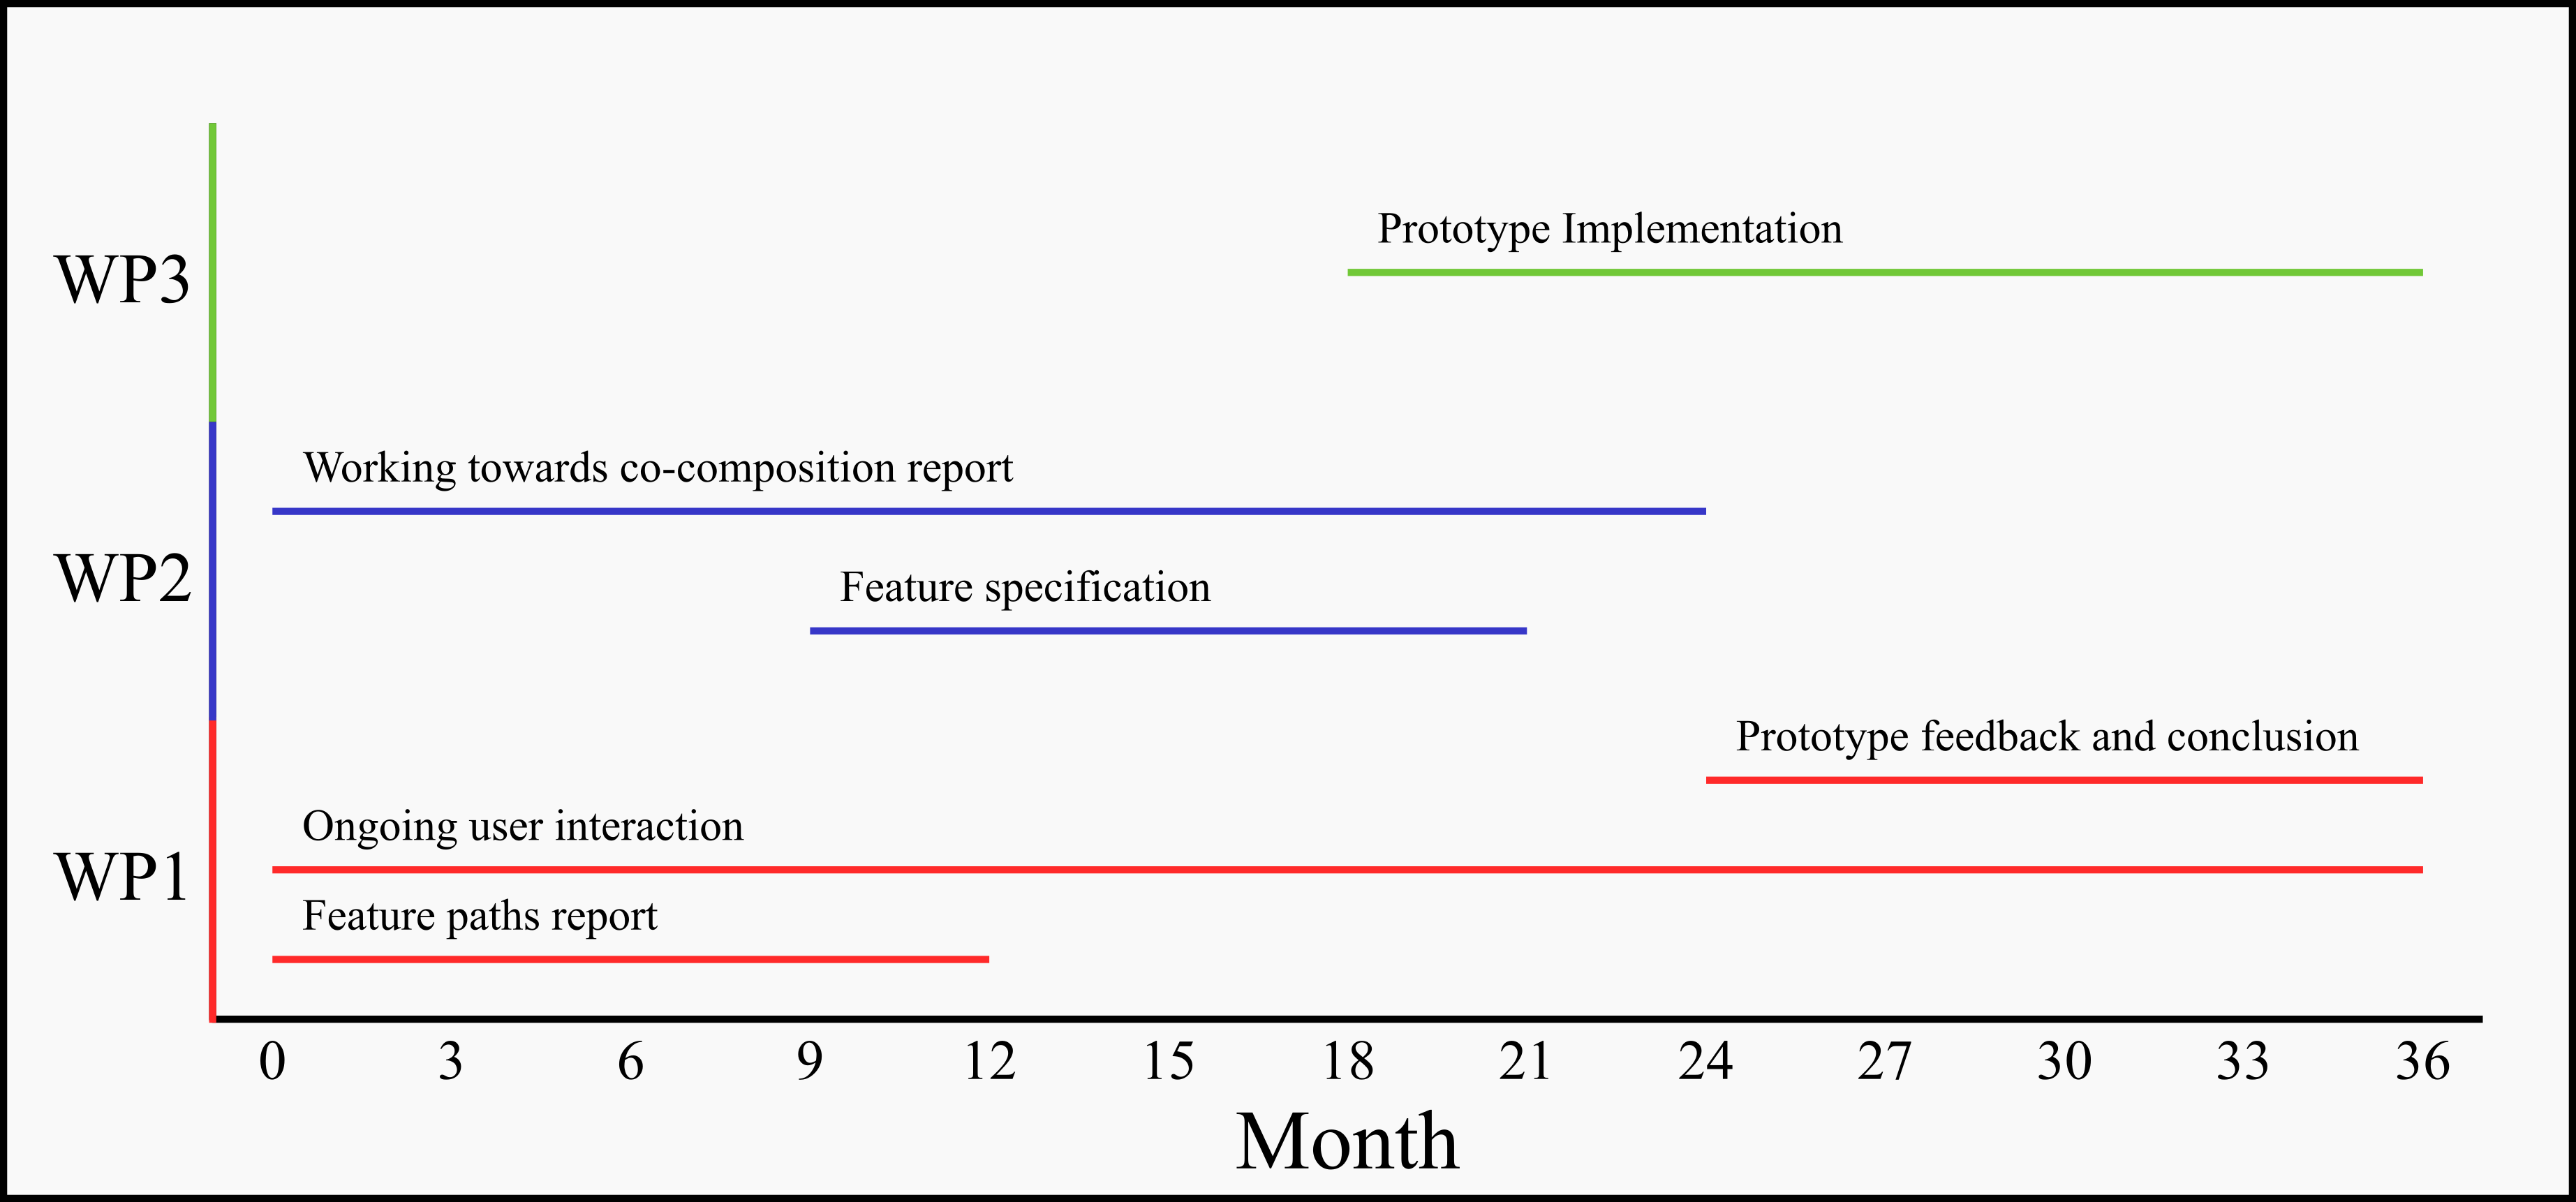
\includegraphics[width=1.0\textwidth]{gantt}
	\end{figure}
	
	\pagebreak6
	\printbibliography
	
\end{document}
